\documentclass[11pt]{article}

\usepackage[margin=1in]{geometry}
\usepackage{graphicx}
\usepackage{xcolor}
\usepackage{listings}
\usepackage{hyperref}
\usepackage{xurl}        % break long URLs at any character
\usepackage[htt]{hyphenat} % allow long \texttt tokens to break
\usepackage{enumitem}
\usepackage{caption}
\usepackage{parskip}

\setlength{\emergencystretch}{3em} % relax justification on stubborn lines

\hypersetup{colorlinks=true, linkcolor=blue!50!black,
  urlcolor=blue!50!black, citecolor=blue!50!black}

\definecolor{codebg}{gray}{0.96}
\definecolor{promptbg}{rgb}{0.95,0.97,1.0}
\lstdefinestyle{code}{basicstyle=\ttfamily\small, backgroundcolor=\color{codebg},
  breaklines=true, frame=single, framerule=0pt, columns=fullflexible,
  showstringspaces=false, xleftmargin=4pt, xrightmargin=4pt}
\lstdefinestyle{prompt}{basicstyle=\ttfamily\small\itshape,
  backgroundcolor=\color{promptbg}, breaklines=true, frame=leftline,
  framerule=2pt, rulecolor=\color{blue!40}, columns=fullflexible,
  xleftmargin=8pt, aboveskip=6pt, belowskip=6pt}
\lstset{style=code}

\lstnewenvironment{prompt}{\lstset{style=prompt}}{}
\newcommand{\fig}[3]{\begin{figure}[ht]\centering
  \includegraphics[width=#2\linewidth]{figures/#1}
  \caption{#3}\label{fig:#1}\end{figure}}

\title{\textbf{Authoring Standards-Conformant HAnim Humanoids with an\\
X3D Model Context Protocol Server: A Human--AI Case Study}}
\author{Alexander Hoffman \and Claude (Anthropic Claude Code)\\[2pt]
  \small\textit{Draft --- collaborative authorship}}
\date{\today}

\begin{document}
\maketitle

\begin{abstract}
We describe the collaborative construction of two interactive 3D demonstrations
---a humanoid running a slalom course and a ``living'' classroom skeleton---built
on the emerging ISO/IEC 19774 (HAnim) Level of Articulation~5 (LOA5) draft and
delivered entirely through an X3D Model Context Protocol (MCP) server driven by a
large language model. Rather than treating the model output as a finished
artifact, we treat the human--AI pair as co-authors: the human supplies intent,
domain pointers, and aesthetic judgment; the AI supplies generation, a tight
verify-by-render feedback loop, and bug-level contributions back to the toolchain.
We report the architecture (X3D MCP, the canonical \texttt{x3d.py} package, the
\texttt{X3dToX3dom.xslt} stylesheet, and the X\_ITE web player), a chronological
case study of the prompting that produced the demos, the practices that made it
reliable, and concrete findings---including upstream bug reports and a roadmap
for layering anatomy (clothing, ligaments, muscles, organs, skin) atop the
skeleton.
\end{abstract}

\section{Introduction}

The popular framing ``the AI built this'' is both inaccurate and uninteresting.
What actually produces good work is a \emph{pairing}: a human who knows where the
problem and the standards live, and a model that can generate, verify, and
iterate at speed. This paper is a worked example. Over a single extended session,
a human collaborator and an AI agent (Anthropic's Claude, running in Claude Code)
built two interactive X3D scenes featuring a fully articulated human skeleton
conforming to the draft LOA5 level of the ISO/IEC 19774 Humanoid Animation
(HAnim) standard, animated with the standard's own walk/run/jump cycles, and
viewable in a web browser.

The contribution is less the scenes themselves than the \emph{method}: every
artifact was produced through an X3D MCP server, validated against the X3D
schema, and---crucially---visually verified by the agent rendering each scene and
inspecting the resulting image before moving on. That loop, plus a decision to
integrate the canonical standard rather than reinvent it, is what made the output
trustworthy.

\fig{fig_canonical_skeleton.png}{0.55}{The canonical HAnim LOA5 bone-mesh
humanoid (150 joints, 243 individual bone meshes from the Web3D
\texttt{AllBonesLOA5Skeletons} model) rendered in Castle Model Viewer. This same
figure is the actor in both demonstrations.}

\section{Background}

\paragraph{X3D.} Extensible 3D (X3D, ISO/IEC 19775) is the royalty-free ISO
standard for declarative 3D scenes---the successor to VRML. A scene is a graph of
\emph{nodes} (geometry, transforms, lights, sensors, interpolators) connected by
\emph{ROUTEs} that carry events. X3D~4.0 added a physically based rendering (PBR)
material, \texttt{PhysicalMaterial}, and image-based lighting via
\texttt{EnvironmentLight}.

\paragraph{HAnim and LOA.} The Humanoid Animation standard (ISO/IEC 19774)
defines a skeleton as a hierarchy of \texttt{HAnimJoint} nodes, each carrying a
named \texttt{HAnimSegment} that holds geometry. A figure's detail is graded by
\emph{Level of Articulation} (LOA): LOA-0 is a single root; the published 2019
standard tops out at LOA-4 (148 joints). The active draft adds \textbf{LOA5}, and
the Web3D example archive ships an \texttt{AllBonesLOA5Skeletons} model---a
150-joint figure whose segments inline individual bone meshes---together with
standardized Walk, Run, Jump and other motion cycles driven by interpolators.

\paragraph{The MCP.} A Model Context Protocol server exposes tools an LLM can
call. The X3D MCP server used here exposes scene construction, validation
(against the X3D~4.x schema), semantic checks, encoding conversion, and X3DOM
page rendering. The agent calls these tools the way a human would click an
editor's menus, but programmatically and at speed.

\section{Setup: Tools, Installs, and Links}\label{sec:setup}

Everything below is free and open. Commands assume macOS with Homebrew
(\href{https://brew.sh}{brew.sh}); the equivalents on Linux/Windows are
noted where they differ. This is the complete list---nothing else is required.

\paragraph{Core authoring and rendering.}
\begin{itemize}[leftmargin=1.4em, itemsep=2pt]
\item \textbf{Java (OpenJDK)} --- runtime for Saxon and NetBeans.
  \texttt{brew install openjdk}. \href{https://openjdk.org}{openjdk.org}.
\item \textbf{Apache NetBeans} + \textbf{X3D-Edit} --- the standards X3D authoring
  tool (tree editor, schema/DTD validation, conversions). Install NetBeans
  (\texttt{brew install --cask netbeans}; \href{https://netbeans.apache.org}{netbeans.apache.org}),
  then inside it: \emph{Tools $\to$ Plugins $\to$ Available Plugins $\to$ search
  ``X3D-Edit'' $\to$ Install}
  (\href{https://savage.nps.edu/X3D-Edit/}{savage.nps.edu/X3D-Edit}). On JDK~24+
  add \texttt{-J-Djdk.xml.entityExpansionLimit=5000} to \texttt{netbeans.conf}
  so X3D's large DOCTYPE does not trip the XML parser.
\item \textbf{Castle Model Viewer} --- GPU X3D viewer with command-line
  screenshots (\texttt{-{}-screenshot}).
  \href{https://castle-engine.io/castle-model-viewer}{castle-engine.io/castle-model-viewer}
  (download the build for your OS; on macOS run \texttt{xattr -cr} on the app to
  clear the quarantine flag).
\end{itemize}

\paragraph{Generation and conversion (the canonical pipeline).}
\begin{itemize}[leftmargin=1.4em, itemsep=2pt]
\item \textbf{x3d.py} --- the official Web3D Python package.
  \texttt{pip install x3d}. \href{https://www.web3d.org/x3d/stylesheets/python/python.html}{web3d.org \dots/python}.
\item \textbf{Saxon-HE} --- an XSLT~2.0 processor (the standard X3D stylesheets
  are XSLT~2.0, which the common \texttt{xsltproc}/libxslt cannot run). Fetch the
  self-contained jar:
\begin{lstlisting}
curl -L -o saxon9he.jar \
  https://repo1.maven.org/maven2/net/sf/saxon/Saxon-HE/9.9.1-8/Saxon-HE-9.9.1-8.jar
\end{lstlisting}
\item \textbf{X3dToX3dom.xslt} --- the official stylesheet that wraps an X3D scene
  into a web page for a chosen player.
  \href{https://www.web3d.org/x3d/stylesheets/X3dToX3dom.xslt}{web3d.org \dots/X3dToX3dom.xslt}.
\end{itemize}

\paragraph{Web players (no install; loaded from a CDN by the page).}
\begin{itemize}[leftmargin=1.4em, itemsep=2pt]
\item \textbf{X\_ITE} --- a WebGL X3D player with full HAnim support.
  \href{https://create3000.github.io/x_ite/}{create3000.github.io/x\_ite} (script
  via \href{https://www.jsdelivr.com}{jsDelivr}).
\item \textbf{X3DOM} --- the other major WebGL X3D player.
  \href{https://www.x3dom.org}{x3dom.org}. (HAnim limitation noted in
  Section~\ref{sec:findings}.)
\end{itemize}

\paragraph{The HAnim LOA5 assets (from the Web3D example archive).}
The skeleton and motion live at
\href{https://www.web3d.org/x3d/content/examples/HumanoidAnimation/Bones/}{web3d.org \dots/HumanoidAnimation/Bones/}:
\texttt{AllBonesLOA5Skeletons.x3d} (the figure),
\texttt{AllBonesLOA5SkeletonsInlineAnimation.x3d} (Walk/Run/Jump cycles), and the
individual bone meshes the segments inline. The draft standard itself is at
\href{https://www.web3d.org/specifications/X3Dv4Draft/ISO-IEC19774/}{web3d.org/specifications/X3Dv4Draft/ISO-IEC19774}.

\paragraph{Optional: texture generation and paper build.}
\begin{itemize}[leftmargin=1.4em, itemsep=2pt]
\item \textbf{mflux} (textures) --- \texttt{pip install mflux} on Apple Silicon;
  weights download from \href{https://huggingface.co}{Hugging Face} on first run.
  Non-Apple equivalent: FLUX.1 or Stable Diffusion via \texttt{diffusers} or
  ComfyUI, or any hosted image API (Section~\ref{sec:arch}).
\item \textbf{tectonic} (this paper) --- a self-contained \LaTeX{} engine that
  fetches packages on demand. \texttt{brew install tectonic};
  \href{https://tectonic-typesetting.github.io}{tectonic-typesetting.github.io}.
  Any \TeX{} distribution works too.
\item \textbf{poppler} (\texttt{pdftoppm}, to preview the PDF as images) and a
  Chromium-based browser (for headless WebGL screenshots) are conveniences for
  the verify-by-render loop, not requirements.
\end{itemize}

\section{Architecture and Toolchain}\label{sec:arch}

The pipeline separates \emph{generation}, \emph{authoring artifact}, and
\emph{delivery}:

\begin{enumerate}[leftmargin=1.4em]
\item \textbf{Generation --- \texttt{x3d.py}.} The official Web3D Python package
  constructs X3D node objects programmatically and serializes valid XML. Building
  a 150-joint humanoid recursively in code is far more maintainable than string
  templating, and the objects validate by construction.
\item \textbf{Authoring artifact --- the \texttt{.x3d} file.} The authoritative
  scene keeps real HAnim nodes, opens in X3D-Edit (the NetBeans-based authoring
  tool) and desktop players, and validates against the schema.
\item \textbf{Delivery --- the web page.} The canonical \texttt{X3dToX3dom.xslt}
  stylesheet (run through the Saxon XSLT~2.0 processor) produces a browser page.
  For the player we use \textbf{X\_ITE}, which has complete HAnim support and
  renders the real skeleton directly; X3DOM, by contrast, cannot yet render an
  HAnim skeleton (see Section~\ref{sec:findings}).
\end{enumerate}

Two supporting tools proved decisive. \textbf{Castle Model Viewer} (a free,
cross-platform X3D/VRML/glTF viewer from the Castle Game Engine project) renders
X3D on the GPU and---critically---can take a screenshot from the command line,
which is how the agent ``sees'' its work (Section~\ref{sec:practices}).

For textures we used \textbf{mflux}. To unpack the acronyms: \textbf{FLUX.1} is
an open-weights text-to-image diffusion model (from Black Forest Labs);
\textbf{MLX} is Apple's array/machine-learning framework optimized for Apple
Silicon GPUs; and \textbf{mflux} is a Python package that runs FLUX.1 on MLX.
Together they generate an image from a text prompt entirely on a local Mac, with
no cloud service. We used it to produce the classroom's chalkboard and anatomy
posters, applied as \texttt{ImageTexture}s---closing a
generate-image~$\rightarrow$~place-in-3D loop. None of this is Apple-specific in
principle: any text-to-image generator (e.g.\ FLUX.1 or Stable Diffusion via
\texttt{diffusers}/ComfyUI on an NVIDIA GPU, or a hosted image API) substitutes
directly; only the local runner changes.

\fig{fig_flux_blackboard.png}{0.6}{A classroom chalkboard texture generated
locally with mflux (FLUX.1-schnell) from a text prompt, then applied as an
X3D \texttt{ImageTexture}. The image-generation and 3D-authoring loops compose.}

\section{Case Study: A Chronological Build}\label{sec:case}

The demos were not specified up front; they emerged through iteration. The
prompts below are simplified reconstructions that capture the \emph{shape} of the
collaboration.

\subsection{From a stick figure to real HAnim}
The first request was direct:
\begin{prompt}
Let's get a human running animation. Use their LOA skeleton and the X3D MCP to make it run correctly, through a level.
\end{prompt}
An initial figure faked joints with nested \texttt{Transform} nodes. The decision
to switch to \emph{real} \texttt{HAnimJoint}/\texttt{HAnimSegment} nodes---using
the standard joint names and centers from the Web3D archive---made the figure
validate and open correctly in standards tools. A key simplification fell out:
because an \texttt{HAnimJoint}'s rest pose is identity, all segment geometry can
be authored in absolute coordinates and still articulate.

\fig{fig_stick_loa4.png}{0.6}{An early LOA-4 figure with generated stick
geometry, running the slalom course. The gait cadence is synchronized to ground
speed so the feet do not skate.}

\subsection{Adopting the canonical pipeline}
A single pointed question redirected the whole approach:
\begin{prompt}
Did you use the x3d.py export or the stylesheets to get to this?
\end{prompt}
The honest answer was ``neither yet''---generation had been ad-hoc string
templating and the web page a hand-rolled converter. \emph{Lesson: a domain
expert's question is a steering signal; the right response is to name the gap
plainly, not paper over it.} The instruction followed:
\begin{prompt}
Rebuild it on the canonical pipeline.
\end{prompt}
Generation moved to \texttt{x3d.py} and delivery to \texttt{X3dToX3dom.xslt} run
through Saxon. This surfaced real serialization quirks
(Section~\ref{sec:findings}) but produced schema-valid, standards-aligned output
that composes with the rest of the ecosystem.

\subsection{Upgrading to LOA5 and the real bones}
The collaborator located the draft LOA5 model and its standardized animation:
\begin{prompt}
Use AllBonesLOA5 for both projects.
\end{prompt}
We downloaded the 243 individual bone meshes, extracted the canonical 150-joint
humanoid as a reusable fragment, and \emph{embedded} it so its \texttt{hanim\_}
joint DEFs were in scope for our animation ROUTEs. The same figure now stars in
both demos.

\fig{fig_runner_bonemesh.png}{0.85}{The canonical LOA5 bone-mesh skeleton running
the slalom course, driven by our gait routed into the standard joints. Rendered
in Castle Model Viewer.}

\subsection{Look development}
The canonical meshes shipped with old-style Phong materials at very high ambient
reflectance, which flattened all anatomical form under image-based lighting. A
batch pass re-authored them as \texttt{PhysicalMaterial} (metallic~0, matte
roughness), restoring depth:
\begin{prompt}
Do the PBR-material pass for the rendered demo and document it. I'm not concerned with canon --- we are doing our demo. This is about what the MCP can do.
\end{prompt}

\begin{figure}[ht]\centering
  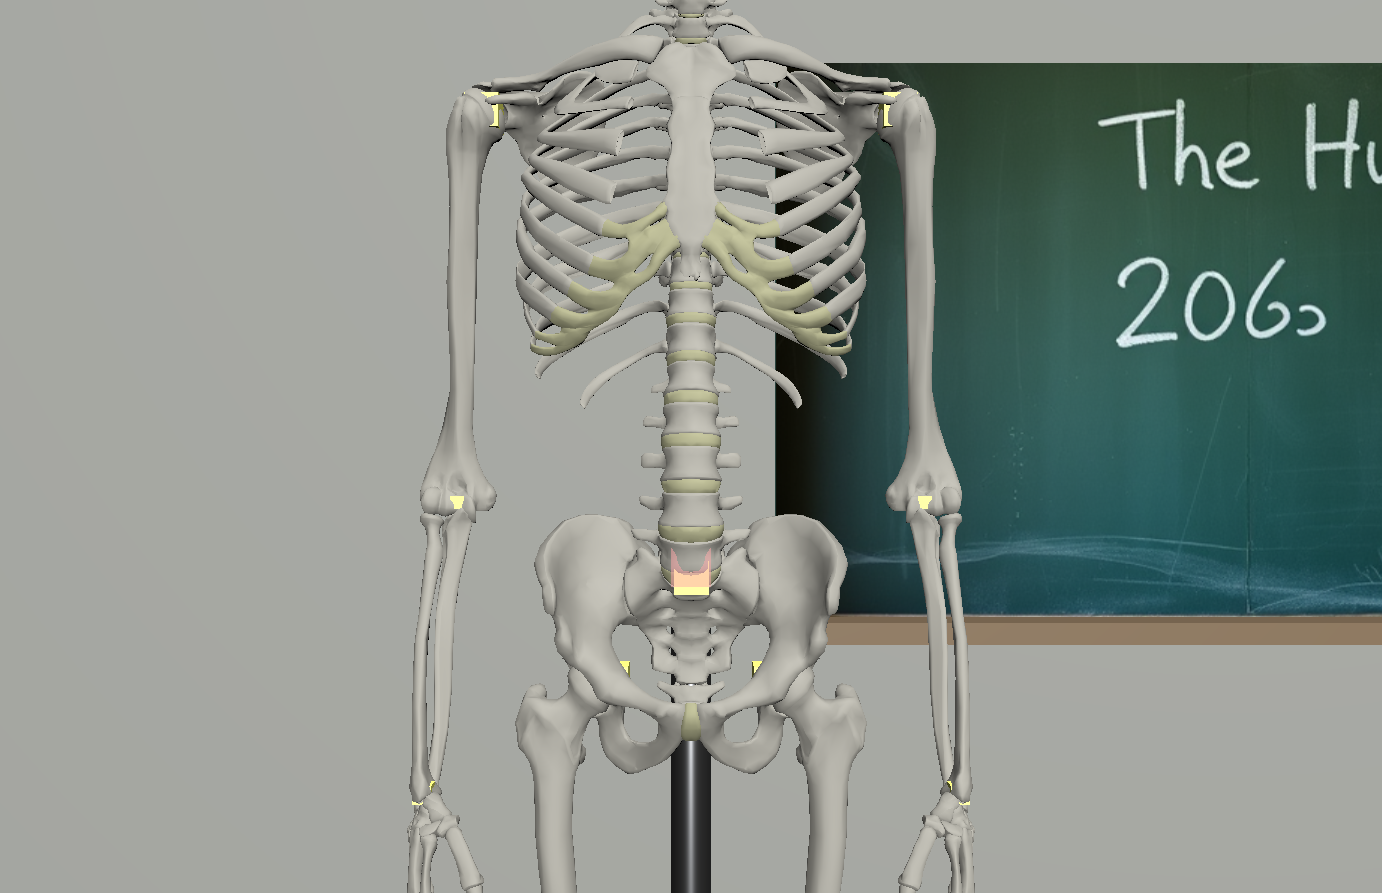
\includegraphics[width=0.6\linewidth]{figures/fig_pbr_torso.png}
  \caption{After the PBR pass: the ribcage, spine, and pelvis recover three
  dimensional form from \texttt{EnvironmentLight}, instead of the flat white wash
  the high-ambient Phong materials produced.}\label{fig:pbr}
\end{figure}

\subsection{Interactivity}
Finally, the classroom skeleton gained the standard's locomotion cycles plus
clickable controls:
\begin{prompt}
Add the LOA5 walk cycles to the classroom. Put buttons on the chalkboard to switch modes.
\end{prompt}
Each cycle (Walk, Run, Jump) was extracted from the standardized animation as a
\texttt{TimeSensor} plus 147 interpolators and routes; an ECMAScript
\texttt{Script} node enables exactly one at a time, triggered by
\texttt{TouchSensor} button panels on the board.

The final shape came from short, corrective prompts---the texture of real
iteration:
\begin{prompt}
Make the skeleton stop waving like that.
\end{prompt}
\begin{prompt}
The buttons should be styled to blend in with the chalkboard.
\end{prompt}
\emph{Lesson: late-stage feedback is mostly aesthetic and behavioral, and it
arrives in small increments. A fast verify-by-render loop
(Section~\ref{sec:practices}) is what lets each one-line note resolve in a single
pass.} These produced the rest pose (arm down) and the chalk-drawn buttons of
Figure~\ref{fig:fig_classroom_buttons.png}.

\fig{fig_classroom_buttons.png}{0.85}{The classroom: the canonical LOA5 skeleton
on a display stand with PBR bones, FLUX-generated chalkboard and posters, and
clickable Walk/Run/Jump/Stand buttons that switch the standardized motion
cycles.}

\section{Practices That Made It Work}\label{sec:practices}

\begin{description}[leftmargin=0pt, style=nextline]
\item[Verify by rendering, not by hoping.] The single most important habit: after
  every change, render the scene to an image and \emph{look}. Castle Model
  Viewer's command-line screenshot mode and a headless WebGL browser let the
  agent catch an invisible humanoid, a neon-glowing skull, a blank chalkboard,
  and washed-out lighting---each of which validated against the schema but looked
  wrong. Schema-valid is not the same as correct.
\item[Integrate the canon; don't reinvent it.] Adopting the official skeleton,
  package, and stylesheet meant the work composed with the broader ecosystem and
  surfaced genuine issues worth reporting upstream.
\item[Separate the authoritative file from the rendered page.] The \texttt{.x3d}
  keeps real HAnim nodes for standards tools; the browser page is generated from
  it. When a player cannot render a construct, adapt the \emph{page}, not the
  source of truth.
\item[Build in stages, commit at each.] Each milestone (skeleton, LOA5, PBR,
  interactivity) was a separate version-control commit, so any step could be
  revisited without losing the others.
\item[Treat tool friction as contribution.] Bugs found while using the tools
  became fixes and reports back to them, not workarounds buried in the demo.
\end{description}

\section{Findings and Contributions}\label{sec:findings}

\begin{itemize}[leftmargin=1.4em]
\item \textbf{MCP fixes.} Using the renderer and validator on real HAnim content
  exposed defects: the X3DOM page renderer crashed on XML comments and failed to
  escape attribute quotes; the semantic checker rejected legal \texttt{set\_}/%
  \texttt{\_changed} ROUTE aliases and flagged conformant \texttt{USE} references
  and empty HAnim joints. These were fixed and submitted upstream.
\item \textbf{\texttt{x3d.py} serialization bugs.} The package omits
  \texttt{containerField} on nodes placed in a non-default field (e.g.\ a joint
  in the \texttt{skeleton} field, a texture in \texttt{baseTexture}), and defaults
  \texttt{EnvironmentLight.global} to \texttt{true} against the spec's
  \texttt{false}. Both yield schema-valid XML that renders wrong. Documented with
  reproductions for the maintainers.
\item \textbf{X3DOM HAnim gap.} Current X3DOM does not render an HAnim skeleton
  and trips a \texttt{MutationObserver} initialization error on large animated
  scenes. X\_ITE renders the same content correctly. This is a concrete
  opportunity to contribute to X3DOM.
\item \textbf{Anatomical-layer roadmap.} The skeleton is a frame to build outward
  from---clothing/coveroids, ligaments, muscles (via \texttt{HAnimDisplacer}
  morphs), organs, nerve/vascular networks, skin (weighted
  \texttt{HAnimHumanoid.skin}), and hair---each a candidate standards
  contribution.
\end{itemize}

\section{Reproducing the Demo}\label{sec:demo}

\begin{enumerate}[leftmargin=1.4em]
\item \textbf{Environment.} Install a JDK, the \texttt{x3d} Python package,
  Saxon-HE (XSLT~2.0), and a viewer (Castle Model Viewer for desktop; a modern
  browser for X\_ITE). Optionally install mflux for texture generation.
\item \textbf{Generate.} Run the generator scripts; each emits an \texttt{.x3d}
  scene and its web page. The skeleton fragment and bone meshes live under
  \texttt{assets/loa5/}.
\item \textbf{Validate.} The scenes pass the X3D~4.0 schema and the MCP semantic
  checker (zero errors).
\item \textbf{View.} Open the \texttt{.x3d} in Castle Model Viewer (or X3D-Edit),
  or open the generated \texttt{.html} in a browser for X\_ITE. In the classroom,
  click \emph{Walk}, \emph{Run}, \emph{Jump}, or \emph{Stand} on the chalkboard
  to switch the figure's motion.
\end{enumerate}

\fig{fig_runner_xite_course.png}{0.85}{The runner demo delivered to the browser
via X\_ITE: the real HAnim figure traverses the slalom course with the
standardized gait. X\_ITE renders the HAnim skeleton directly, with no
flattening.}

\section{Conclusion}

A capable model and a person who knows the domain are stronger together than
either alone, and saying so plainly---``we built this''---is both more accurate
and more useful than the marketing shorthand. The concrete enablers were modest:
expose the toolchain through an MCP, integrate the actual standard, and close a
verify-by-render loop so the agent is accountable to what the scene looks like,
not just whether it parses. The result is a standards-conformant, interactive
LOA5 humanoid demonstration---and a short list of contributions handed back to
the tools that made it.

\end{document}
